\section{Sensitivity to Expert-Memory Capacity (R2-03)}
\label{sec:sensitivity-capacity}

The 4~GiB comparison (Section~\ref{sec:oracle-headroom}) is a single
point. We next test how the Global-LRU-vs-$O_B$ gap behaves across a
fixed, predeclared sweep of five expert-memory budgets --
$1.5, 2, 4, 8, 16$~GiB -- replaying the same declared policy set
(Section~\ref{sec:oracle-headroom}) on the same validated trace at each
budget. The 4~GiB point is a mandatory reproduction anchor: it must
reproduce R2-02's registered Global-LRU and Oracle-Global-Belady ($O_B$)
evidence exactly, and does (Table~\ref{tab:r2-03-sweep}).

\begin{figure}[t]
\centering
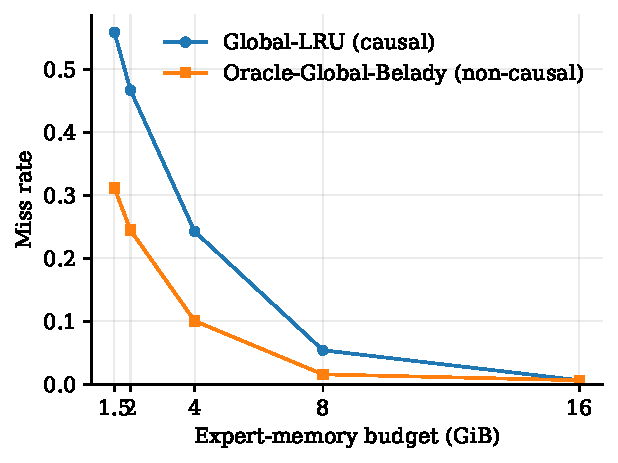
\includegraphics[width=0.72\linewidth]{figures/figure1_miss_rate_vs_budget.pdf}
\caption{Global-LRU (causal) vs.\ Belady comparator $O_B$ (clairvoyant)
miss rate as a function of expert-memory budget (R2-03). Generated by
\texttt{figures/make\_figures.py} from the frozen data snapshot; binary
figure assets were regenerated as presentation artifacts for the
\textsc{AUDIT-ORACLE-001} semantics amendment.}
\label{fig:miss-rate-vs-budget}
\end{figure}

\begin{figure}[t]
\centering
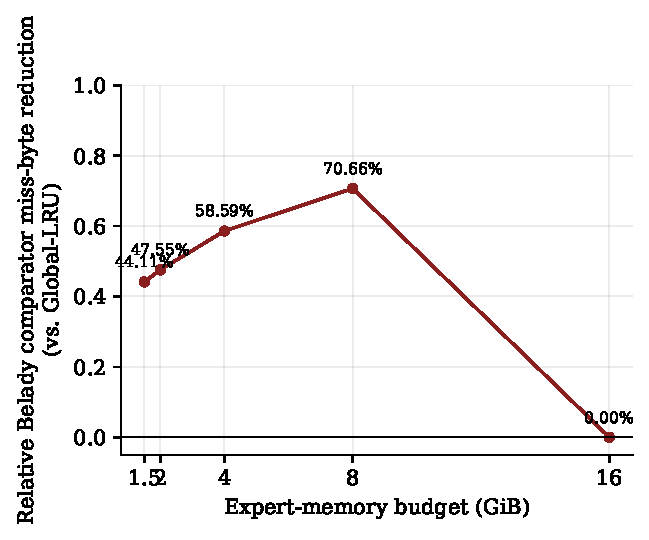
\includegraphics[width=0.72\linewidth]{figures/figure2_relative_headroom_vs_budget.pdf}
\caption{Relative Belady comparator miss-byte reduction over Global-LRU
($G_\budget(\text{Global-LRU},O_B)$, Definition~\ref{def:comparator-gap})
as a function of expert-memory budget (R2-03). The curve rises across the
capacity-constrained points tested ($1.5$--$8$~GiB) and collapses to
zero at $16$~GiB, the first tested budget at which the expert working set
becomes effectively resident. This is a measured comparator gap, not a
proven causal-recovery upper bound.}
\label{fig:headroom-vs-budget}
\end{figure}

\begin{table}[t]
\centering
\caption{Global-LRU vs.\ Oracle-Global-Belady across the tested expert-memory budget sweep (R2-03).}
\label{tab:r2-03-sweep}
\small
\begin{tabular}{@{}rrrrr@{}}
\toprule
Budget (GiB) & Global-LRU misses & Oracle misses & Rel.\ miss-byte reduction & Abs.\ miss-byte reduction (GB) \\
\midrule
1.5 & 81,752 & 45,603 & 44.11\% & 103.57 \\
2 & 68,318 & 35,821 & 47.55\% & 93.42 \\
4 & 35,529 & 14,754 & 58.59\% & 59.86 \\
8 & 7,952 & 2,350 & 70.66\% & 16.18 \\
16 & 973 & 973 & 0.00\% & 0.00 \\
\bottomrule
\end{tabular}
\end{table}


\paragraph{Monotonicity and collapse.} Across the four capacity-constrained
tested points ($1.5$--$8$~GiB, where Global-LRU incurs a nonzero eviction
count), the relative Belady comparator gap rises from $44.11\%$ at
$1.5$~GiB to its largest tested relative value of $70.66\%$ at $8$~GiB.
The largest tested absolute comparator gap among tested points is
$103.57$~GB at $1.5$~GiB. At $16$~GiB, Global-LRU and $O_B$ produce
\emph{identical} miss counts, miss bytes, and zero evictions each: the
expert working set is effectively resident at this budget for the tested
workload, and neither the causal baseline nor the clairvoyant comparator
has evictions to decide. We term $16$~GiB the \emph{first tested
policy-indifference budget}; this is an empirical statement about the
five tested points, not a claim about the mathematically minimal
capacity at which convergence occurs (which may be lower; it was not
swept at finer granularity above $8$~GiB).

\paragraph{Non-monotonic structural gap.} Unlike the comparator gap, the
\emph{structural} Runtime-Sharded-LRU-vs-Global-LRU gap is not monotonic
across the sweep: it is slightly \emph{negative} at $1.5$ and $2$~GiB
(sharding itself reduces miss bytes by $1.82\%$ and $0.39\%$ respectively,
relative to Global-LRU) and positive at $4$ and $8$~GiB ($1.16\%$ and
$2.61\%$). This sign change is a valid observed result
(Section~\ref{sec:recoverable-envelope}) and is not forced to any
particular shape.
